\section{Das primale Simplex-Verfahren}

Das primale Simplexverfahren durchläuft zwei Phasen (falls nötig):
\begin{itemize}
	\item Phase 1 besteht aus der Ermittlung einer ersten Ecke (zulässige Basislösung), 
	\item Phase 2 aus der darauf aufbauenden Bestimmung einer optimalen Ecke.
\end{itemize} 

\subsection{Phase 2 des Simplex-Verfahrens}

Wir betrachten die (erste) zulässige Basislösung (Ecke) $x = (x_B, x_N)$ und schreiben \eqref{eq: 3.3} als Simplex-Tableau:

\begin{center}
	\begin{tabular}{r|c|c}
		$T_0$ & $x_N$ & $1$ \\ \hline
		$x_B = $ & $P$ & $p$ \\ \hline
		$z =$ & $\trans{q}$ & $q_0$
	\end{tabular}
\end{center}

\begin{equation}
	\begin{aligned}
		P &= -A_B^{-1} A_N  &
		p &= A_B^{-1} b \\
		\trans{q} &= \trans{c_N} - \trans{c_B} A_B^{-1} A_N &
		q_0 &= \trans{c_B} A_B^{-1} b 
	\end{aligned}
	\label{eq: 3.5}	
\end{equation}

%Optimalität erkenn man nun an der Bedingung $\trans{q} \ge 0$.

Wir nehmen zunächst an, dass $x = (x_B, x_N)$ eine nicht-entartete Ecke mit $x_B = \transpose{x_1, \dots, x_m}$ und $x_N = \transpose{x_{m+1}, \dots, x_n}$ ist. Die hierzu gehörige Basislösung ist $x = (x_B, x_N) = (p,0)$ und es gilt $p \ge 0$ (da zulässig). Folglich ist $x \in G$.

\textbf{Frage:} Wenn $x$ nicht optimal ist -- wie kann eine bessere zulässige Basislösung (Ecke) gefunden werden?

\textbf{Antwort:} Wahl einer zulässigen Richtung $d \in Z(x)$ mit maximaler Schrittweite, die eine Verkleinerung des Zielfunktionswerts ermöglicht.

Nach \cref{aussage: 3.4} ist $x$ optimal, falls $q \ge 0$ gilt. Sei nun $q_\tau < 0$ für $\tau \in I_N$. Zur Konstruktion einer neuen Ecke setzen wir $x_\tau = t$ (bisher war $x_\tau = 0$). Dann folgt zunächst $x_N(t) = t * e_\tau$ und wegen der Forderung $x_N(t) \ge 0$ auch $t \ge 0$. Ferner ergibt sich aus Tableau $T_0$ der Zusammenhang $x_i(t) = P_{i \tau} * x_\tau + p_i = P_{i \tau} * t + p_i$ für alle $i \in I_B$.

Insgesamt verfolgen wir ausgehend von $x =(p,0)$ die zulässige Richtung $d \in \Rn$
\begin{equation*}
	d_i = \begin{cases}
	P_{i \tau} & i \in I_B \\
	1 & i = \tau \\
	0 & i \in I_N \setminus \menge{\tau}
\end{cases}
\end{equation*}

Die maximale Schrittweite $\quer{t}$ erhält man wie folgt: Für jedes $i \in I_B$ ist $x_i(t) \ge 0$ zu gewährleisten. Gilt $P_{i \tau} \ge 0$, so ergibt dies keine Einschränkung für die Schrittweite (weil $p_i \ge 0$, $t \ge 0$, $P_{i \tau} \ge 0$ $\follows x_i(t) \ge 0$ für alle $t \ge 0$). Für $P_{i \tau} < 0$ muss hingegen $t \le - \frac{p_i}{P_{i \tau}}$ (aus Tableauzusammenhang) gewählt werden. Die maximal mögliche Schrittweite ergibt sich folglich zu
\begin{equation}
t \le \quer{t} = \quer{t}(x,d) \defeq \min\menge{- \frac{p_i}{P_i \tau} \colon P_{i \tau} < 0, i \in I_B}
\label{eq: 3.6}
\end{equation}
bzw. $\quer{t} = \infty$, falls $P_{i \tau} \ge 0$ für alle $i \in I_B$.

\begin{aussage} %3.5
	Im Fall $\quer{t} = \infty$ besitzt \eqref{eq: 3.1} keine Lösung, da die Zielfunktion nach unten unbeschränkt ist.
\end{aussage}
\begin{proof}
	Wegen $\quer{t} = \infty$ gilt $x(t) \in G$ für alle $t \ge 0$. Dann liefert $q_\tau < 0$ sogleich $Z(t) = \quer{q} * x_N(t) + q_0 \overset{x_N(t) = t * e_\tau}{=} q_\tau * t + q_0 \to - \infty$ für $t \to \infty$.
\end{proof}

\begin{bemerkung} %3.2
	Die beiden Fälle 
	\begin{enumerate}[nolistsep, topsep=-\parskip]
		\item $q_i \ge 0$ für alle $i \in I_N \qquad \leadsto$ Optimalität
		\item es existiert ein $\tau \in I_N$ mit $q_\tau < 0$ und $P_{i \tau} \ge 0$ für alle $i \in I_B \qquad \leadsto$ Unbeschränktheit
	\end{enumerate}
	werden primal entscheidbar genannt.
\end{bemerkung}

Im sogenannten nicht-entscheidbaren Fall, d.h. falls
\begin{equation*}
	\brackets{\exists \ \tau \in I_N \colon a_\tau < 0} \land \brackets{ \exists \ \sigma \in I_B \colon \quer{t} = -\frac{p_\sigma}{P_{\sigma \tau}} = \min \menge{-\frac{p_i}{P_{i \tau}} \colon P_{i \tau} < 0, i \in I_B} < \infty}
\end{equation*}
ergibt die (maximale) Schrittweite $\quer{t}$ den Punkt
\begin{equation*}
	\quer{x} = x + \quer{t} d \in G \mit f(\quer{x}) = f(x) + \quer{t} q_\tau = q_0 + \quer{t} q_\tau
\end{equation*}
Für entartete Ecken kann man die Schrittweite $\quer{t} = 0$ erhalten. In diesem Fall ändert sich der Punkt $\quer{x}$ nicht, aber die Menge $I_N$ und $I_B$. Zum Verlassen einer (noch nicht optimalen) entarteten Ecke können mehrere Schritte nötig sein. 

\begin{satz} %3.6
	\label{satz: 3.6}
	$\quer{x}$ ist eine Ecke von $G$ mit Basis-Indexmenge
	\begin{equation*}
		\begin{aligned}
			\quer{I_B} &= \quer{I_B}(\quer{x}) \defeq \brackets{I_B \setminus \menge{\sigma}} \cup \menge{\tau} \\
			\quer{I_N} &= \quer{I_N}(\quer{x}) \defeq \brackets{I_N \setminus \menge{\tau}} \cup \menge{\sigma}
		\end{aligned}
	\end{equation*}
\end{satz}

Um zu zeigen, dass die Matrix $\quer{A_B} \defeq \brackets{A^i}_{i \in \quer{I_B}}$ regulär ist, nutzen wir das folgende Resultat.

\begin{lemma}[Sherman / Morrison] %3.7
	\label{lemma: 3.7}
	Es seien $B \in \R^{m \times m}$ regulär und $u,v \in \Rm$. Die Matrix $\quer{B} \defeq B + u \trans{v}$ ist genau dann regulär, wenn $1 + \trans{v} B^{-1} u \neq 0$ erfüllt ist und dann gilt
	\begin{equation*}
		\quer{B}^{-1} = B^{-1} - \frac{B^{-1} u \trans{v} B^{-1}}{1 + \trans{v} B^{-1} u}
	\end{equation*}
\end{lemma}
\begin{proof}
	Übung oder Selbststudium (aber wird nie gefragt werden)
\end{proof}

\begin{proof}[\cref{satz: 3.6}]
	Der ''Austausch`` der Spalten $A^\tau$ und $A^\sigma$ kann durch ein dyadisches Produkt $u \trans{v}$ beschrieben werden:
	\begin{equation*}
		\quer{A_B} = A_B + u \trans{v} \mit u = A^\tau - A^\sigma \und v = e^\sigma 
	\end{equation*}
	Wegen
	\begin{align*}
		1 + \trans{v} B^{-1} u &= 1 + \transpose{e^\sigma} A_B^{-1} \brackets{A^\tau - A^\sigma} \\ 
		&= 1 + \transpose{e^\sigma} A_B^{-1} A^\tau - 1 \tag{''$A^\sigma \in A_B$``} \\
		&= - P_{\sigma \tau} \neq 0
		\tag{$P = -A_B^{-1}A_N$ und ''$A^\tau \in A_N$``}
	\end{align*}
	folgt aus \cref{lemma: 3.7} die Regularität von $\quer{A_B}$.
\end{proof}

\begin{beispiel} %3.2
	\label{beispiel: 3.2}
	Wir betrachten die lineare Optimierungsaufgabe
	\begin{equation*}
		z = -x_1 - x_2 \to \min \bei x_1 + 2 x_2 \le 6, 4x_1 + x_2 \le 10, x_1, x_2 \ge 0
	\end{equation*} 
	Um aus den Ungleichungen Gleichungsnebenbedingungen zu machen, führen wir sogenannte \begriff{Schlupfvariablen} $x_3, x_4 \ge 0$ ein und erhalten
	\begin{equation*}
		\begin{alignedat}{3}
			x_1 + 2 x_2 + x_3 &= 6, &\quad  4x_1 + x_2 + x_4 &= 10, &\quad x_1, x_2, x_3, x_4 &\ge 0 \\
			\follows \qquad \qquad \qquad x_3 &= 6 - x_1 - 2x_2, & \quad x_4 &= 10 - 4x_1 + x_2 &&
		\end{alignedat}
	\end{equation*}
	Damit liegt nun eine Optimierungsaufgabe in Standardform \eqref{eq: 3.1} vor. Notieren wir dies nun in Tableauform mit $I_N = \menge{1,2}$ und $I_B = \menge{3,4}$ (betrachte dazu $x_B = Px_N + p$):	
	\begin{center}
		\begin{tabular}{r|cc|c l}
			$T_0$ & $x_1$ & $x_2$ & $1$ \\ \cline{1-4}
			$x_3 = $ & $-1$ & $-2$ & $6$ & {\footnotesize $\quer{t} = \frac{6}{1}$} \\ 
			$x_4 = $ & $-4$ & $-1$ & $10$ & {\footnotesize $\quer{t} = \frac{10}{4}$} \\ \cline{1-4}
			$z =$ & $-1$ & $-1$    & $0$
		\end{tabular}
	\end{center}
	Wir können nun $\tau \in \menge{1,2}$ wählen, oBdA wählen wir hier $\tau = 1$.
	Für $x_3$ ergibt sich eine maximale Schittweite $\quer{t} = -\frac{p_i}{P_{i \tau}} = \frac{6}{1}$. Für $x_4$ ergibt sich $\quer{t} = \frac{10}{4}$.  Damit wird $\sigma = 4$ gewählt.
	
	Mit $\tau = 1$ und $\sigma = 4$ sowie $\quer{t} = \frac{5}{2}$ erhält man
	\begin{equation*}
		\quer{x} = x + \quer{t} d = \left( \begin{smallmatrix} 0 \\ 0 \\ 6 \\ 10 \end{smallmatrix} \right) + \frac{5}{2} \left( \begin{smallmatrix} 1 \\ 0 \\ -1 \\-4 \end{smallmatrix} \right)
		= \left( \begin{smallmatrix} \frac{5}{2} \\ 0 \\ \frac{7}{2} \\ 0 \end{smallmatrix} \right)
		\quad \und \quad 
		z(\quer{x}) = -\frac{5}{2}
	\end{equation*}
\end{beispiel}

Der Austausch von $x_\tau$ und $x_\sigma$ im Simplextableau kann formal durch die sogenannten Austauschregeln erfolgen.

\begin{center}
	\begin{minipage}{\dimexpr0.6\linewidth-\fboxrule-\fboxsep}
		\centering
		\begin{tabular}{r|c|c}
			$T_0$ & $x_N$ & $1$ \\ \hline
			$x_B = $ & $P$ & $p$ \\ \hline
			$z =$ & $\trans{q}$ & $q_0$
		\end{tabular}
		$\quad \implies \quad$
		\begin{tabular}{r|c|c}
			$T_1$ & $x_{\schlange{N}}$ & $1$ \\ \hline
			$x_{\schlange{B}} = $ & $\schlange{P}$ & $\schlange{p}$ \\ \hline
			$z =$ & $\trans{\schlange{q}}$ & $\schlange{q_0}$
		\end{tabular}
	\end{minipage}
	\begin{minipage}{\dimexpr0.4\linewidth-\fboxrule-\fboxsep}
		\begin{equation*}
			\begin{aligned}
			\schlange{I_B} &= \brackets{I_B \cup \menge{\tau}} \setminus \menge{\sigma} \\
			\schlange{I_N} &= \brackets{I_B \cup \menge{\sigma}} \setminus \menge{\tau}
			\end{aligned}
		\end{equation*}
	\end{minipage}
\end{center}
\vspace{\parskip}

\fbox{Austauschregeln:}
\begin{align*}
	\schlange{P}_{\sigma , \tau} &\defeq \frac{1}{P_{\sigma,  \tau}} 
	\tag{Pivotelement} \\
	%
	\schlange{P}_{\sigma, j} &\defeq - \frac{P_{\sigma, j}}{P_{\sigma, \tau}} \quad (j \in I_N \setminus \menge{\tau}) & \schlange{p}_\sigma &= - \frac{p_\sigma}{P_{\sigma, \tau}} 
	\tag{Pivotzeile} \\
	%
	\schlange{P}_{i, \tau} &\defeq - \frac{P_{i, \tau}}{P_{\sigma, \tau}} \quad (i \in I_B \setminus \menge{\sigma}) & \schlange{q}_\tau &\defeq \frac{q_\tau}{P_{\sigma, \tau}}
	\tag{Pivotspalte} \\
	%
	\schlange{P}_{i,j} &\defeq P_{i,j} - \frac{P_{\sigma, j}}{P_{\sigma, \tau}} P_{i,\tau} \quad (i \in I_B \setminus \menge{\sigma} , j \in I_N \setminus \menge{\tau}) 
	\tag{sonstige Elemente}\\
	%
	\schlange{p}_i &\defeq p_i - \frac{p_\sigma}{P_{\sigma, \tau}} P_{i,\tau} \quad (i \in I_B \setminus \menge{\sigma}) \\
	\schlange{q}_j &\defeq q_j - \frac{P_{\sigma, j}}{P_{\sigma, \tau}} q_\tau \quad (j \in I_N \setminus \menge{\tau}) \\
\end{align*}

Vergleiche dazu auch das Merkblatt zum Simplex-Verfahren unter auf den folgenden Seiten. 

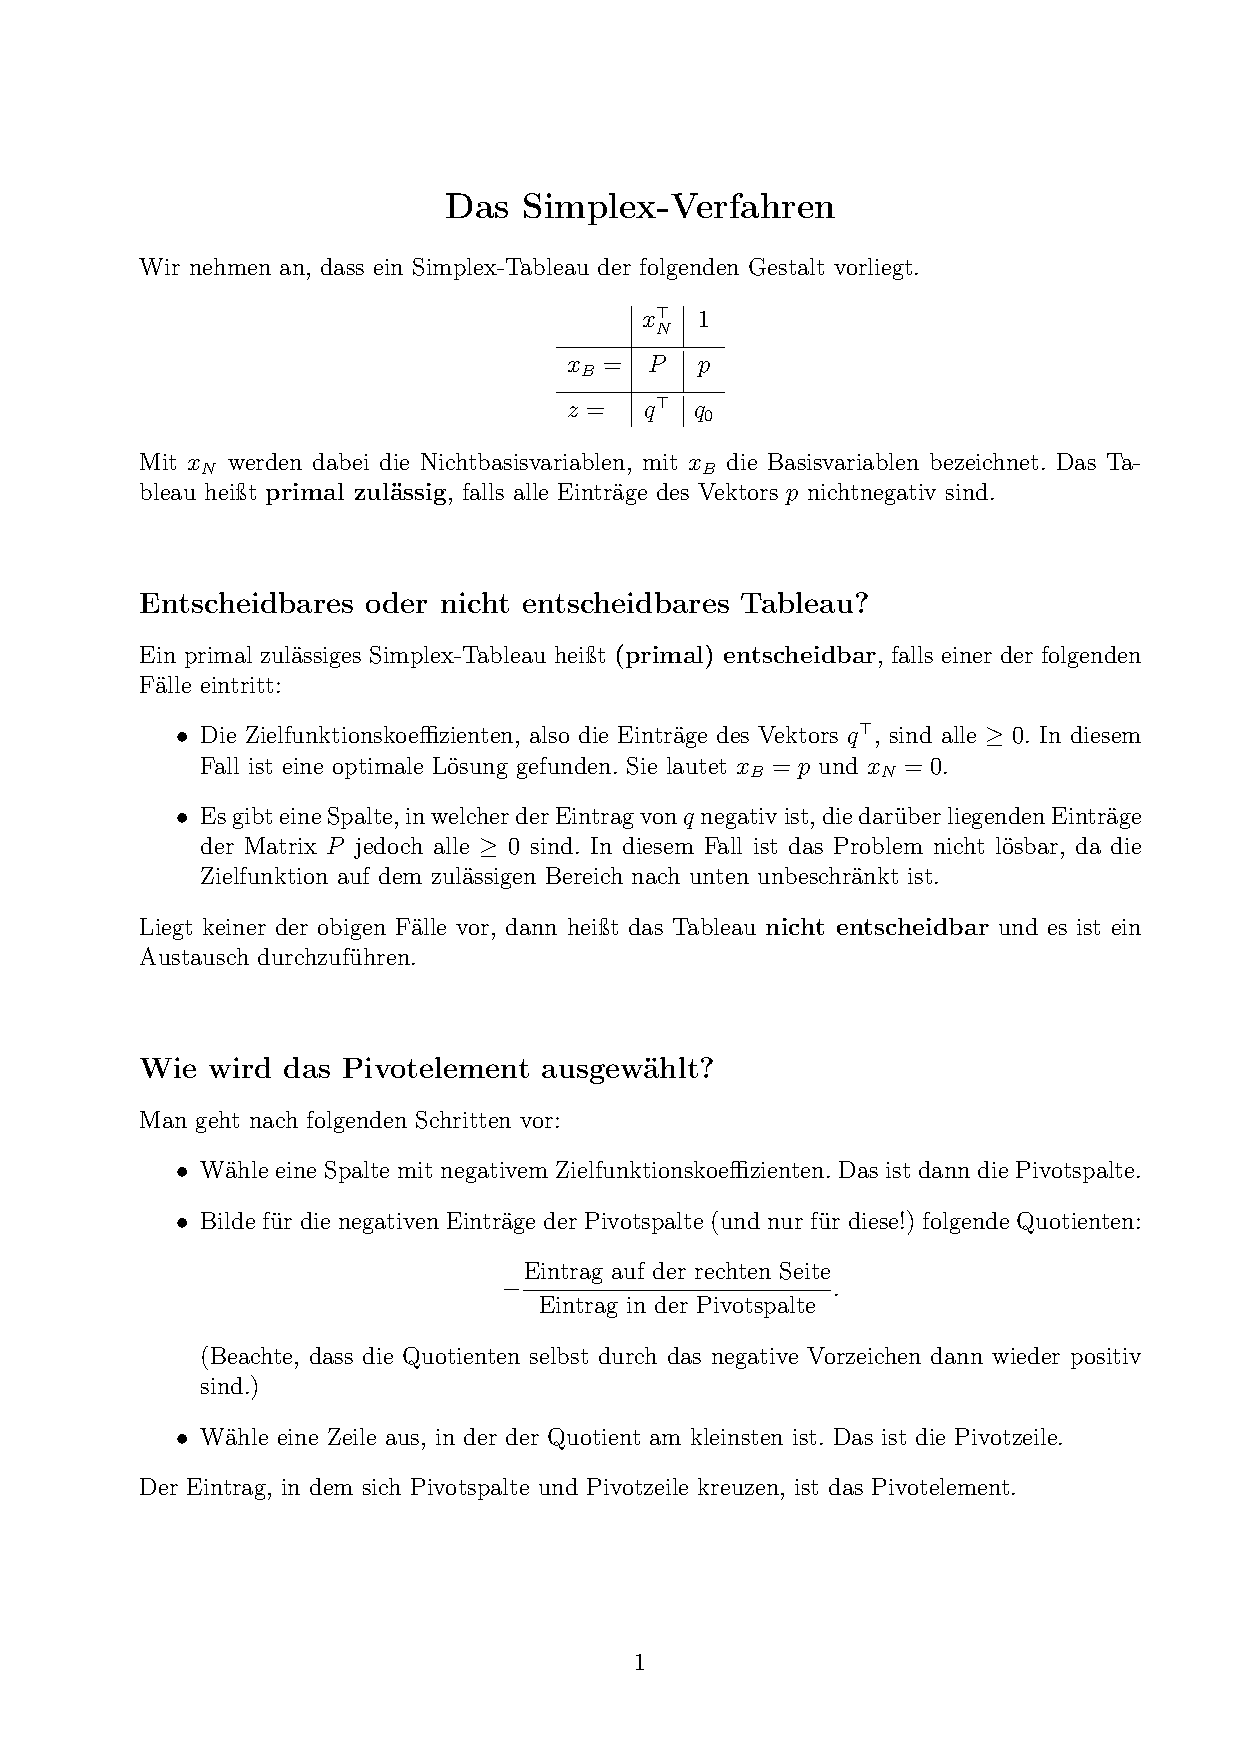
\includepdf[pages=-]{optinum_zsfSimplex.pdf}

\begin{beispiel} %3.3
	Wir betrachten wie in \cref{beispiel: 3.2} die Optimierungsaufgabe
	\begin{equation*}
	z = -x_1 - x_2 \to \min \quad \bei \quad x_1 + 2 x_2 \le 6, \enskip 4x_1 + x_2 \le 10, \enskip x_1, x_2 \ge 0
	\end{equation*} 
	mit Simplex-Starttableau:
	\begin{indentpar}
		\begin{tabular}{R{1.8cm}|R{0.6cm}R{0.6cm}|R{0.6cm} l}
			$T_0$ & $x_1$ & $x_2$ & $1$ \\ \cline{1-4}
			$x_3 = $ & $-1$ & $\fbox{-2}$ & $6$ & {\footnotesize $\quer{t} = 3$} \\ 
			$x_4 = $ & $-4$ & $-1$ & $10$ & {\footnotesize $\quer{t} = 10$} \\ \cline{1-4}
			$z =$ & $-1$ & $-1$    & $0$ \\ \cline{1-4}
			Kellerzeile & $-\frac{1}{2}$ & $\ast$ & $3$ & {\footnotesize = neue Pivotzeile}
		\end{tabular}
	\end{indentpar}
	Nun wählen wir aber $\tau = 2$, woraus sich $\sigma =  3$ ergibt.
	Zur besseren Übersicht haben wir eine Kellerzeile eingeführt. Diese entspricht genau der neu berechneten Pivotzeile.
	\begin{indentpar}
		\begin{tabular}{R{1.8cm}|R{0.6cm}R{0.6cm}|R{0.6cm} l}
			$T_1$ & $x_1$ & \textcolor{cdpurple}{$x_3$} & $1$ \\ \cline{1-4}
			\textcolor{cdpurple}{$x_2 = $} & $- \sfrac{1}{2}$ & $-\sfrac{1}{2}$ & $3$ & {\footnotesize (Division durch -1 * Pivot)} \\ 
			$x_4 = $ & $-\sfrac{7}{2}$ & $\sfrac{1}{2}$ & $7$ \\ \cline{1-4}
			$z =$ & $-\sfrac{1}{2}$ & $\sfrac{1}{2}$  & $-3$ \\ \cline{1-4}
			Kellerzeile & $-\sfrac{2}{7}$ & $\sfrac{1}{7}$ & $2$
		\end{tabular}
	\end{indentpar}
	Nebenrechnung: z.B. $ 7 = 10 + 3 * (-1)$
	
	Im nächsten Schritt wählen wir nun $\tau = 1$ und $\sigma = 4$.
	\begin{indentpar}
		\begin{tabular}{R{1.8cm}|R{0.6cm}R{0.6cm}|R{0.6cm} l}
			$T_2$ & \textcolor{cdpurple}{$x_4$} & $x_3$ & $1$ \\ \hline
			$x_2 = $ & $\sfrac{1}{7}$ & $-\sfrac{4}{7}$ & $2$ & \\ 
			\textcolor{cdpurple}{$x_1 = $} & $-\sfrac{2}{7}$ & $\sfrac{1}{7}$ & $2$ \\ \hline
			$z =$ & $\sfrac{1}{7}$ & $\sfrac{3}{7}$  & $-4$ 
		\end{tabular}
	\end{indentpar}
	Da $\schlange{p} = \brackets{\begin{smallmatrix} 2 \\ 2 \end{smallmatrix}} \ge 0$ ist, ist die Lösung zulässig. Außerdem wissen wir wegen $\trans{\schlange{q}} = \brackets{\sfrac{1}{7}, \sfrac{3}{7}} \ge 0$, dass die Lösung optimal ist. Somit ergibt sich
	\begin{equation*}
		x^\ast = (x_1^\ast, x_2^\ast, x_3^\ast, x_4^\ast) = (2,2,0,0) \mit z^\ast = -4
	\end{equation*}
\end{beispiel}

\subsection{Phase 1 (Hilfsfunktionsmethode)}

Wir betrachten das Problem
\begin{equation}
	z = \trans{c} x \to \min \bei Ax = b , x \ge 0
	\label{eq: 3.7}
\end{equation}
Ohne Einschränkung sei $b \ge 0$. Durch folgendes Hilfsproblem lässt sich eine Startecke ermitteln (sofern eine solche überhaupt existiert). 
\begin{equation}
	h = \trans{e} y \to \min \bei y + Ax = b, x \in \Rn_+, y \in \Rm_+
	\label{eq: 3.8}
\end{equation}
mit $e = \transpose{1, \dots , 1} \in \Rm$.
Eine erste Basislösung für \eqref{eq: 3.8} ist gegeben durch 
\begin{equation}
	\begin{array}{@{}r|c|c@{}}
		T_0 & x & 1 \\ \hline
		y =  & -A & b \\ \hline
		h = & -\trans{e}A & \trans{e} b
	\end{array}
	\label{eq: 3.9}
\end{equation}

\begin{satz} %3.8
	Das Problem \eqref{eq: 3.7} besitzt genau dann eine zulässige Lösung, wenn $h_{\min} = 0$ den Optimalwert von \eqref{eq: 3.8} darstellt.
\end{satz}
\begin{proof}
	Offenbar gilt $h_{\min} = 0 \equivalent y = 0$.
	\begin{proof-equivalence}
		\hinrichtung Besitzt \eqref{eq: 3.7} eine zulässige Lösung $\schlange{x}$, dann ist $\left( \begin{smallmatrix} \schlange{x} \\ 0 \end{smallmatrix} \right)$ zulässig für \eqref{eq: 3.8}. Wegen $0 \le h = \trans{e} \schlange{y} = 0$ folgt $h_{\min} = 0$.
		\rueckrichtung Hat man umgekehrt $h_{\min} = 0$, so gilt $\schlange{y} = 0$ für jede optimale Lösung $\left( \begin{smallmatrix} \schlange{x} \\ \schlange{y} \end{smallmatrix} \right)$ von \eqref{eq: 3.8}. Aus der Zulässigkeit von $\left( \begin{smallmatrix} \schlange{x} \\ \schlange{y} \end{smallmatrix} \right)$ für \eqref{eq: 3.8} folgt dann die Zulässigkeit von $\schlange{x}$ für \eqref{eq: 3.7}.
	\end{proof-equivalence}
\end{proof}

\subsection{Der Simplexalgorithmus}

Mit den zuvor beschriebenen Vorgehensweisen lässt sich das Simplexverfahren zur Lösung der Optimierungsaufgabe \eqref{eq: 3.1} wie folgt algorithmisch formulieren:
\begin{itemize}
	\item \textbf{Schritt 1} (\textit{Initialisierung}): Ermittle eine erste zulässige Basislösung $x = \transpose{\trans{x_B}, \trans{x_N}} = \transpose{\trans{p}, \trans{0}}$ mit $p = (A_B)^{-1} b \ge 0$, wobei $I_B$ die Menge der Basisindizes ist und stelle ein erstes Simplextableau auf.
	\item \textbf{Schritt 2} (\textit{Optimalitätstest}): Berechne entsprechend \cref{aussage: 3.4}
	\begin{equation}
		\quer{q} \defeq \min_{j \in I_N} q_j \quad \mit \quad q_J \defeq c_j \trans{d} A^j \enskip (j \in I_N)
		\label{eq: 3.10}
	\end{equation}
	wobei $\trans{d} \defeq \trans{c_B} (A_B)^{-1}$ ist. Gilt $\quer{q} \ge 0$, dann ist $x$ Lösung von \eqref{eq: 3.1}. Andernfalls sei $q_\tau = \quer{q} < 0$.
	\item \textbf{Schritt 3} (\textit{Test auf Unbeschränktheit}): Gilt $P_{i \tau} \ge 0$ für alle $I \in I_B$, so ist die Aufgabe nicht lösbar ($f^\ast = -\infty$).
	\item \textbf{Schritt 4} (\textit{Austauschschritt}): Bestimme die Pivotzeile $\sigma$ gemäß
	\begin{equation*}
		- \frac{p_\sigma}{P_{\sigma \tau}} = \min \menge{- \frac{p_i}{P_{i \tau}} \colon \quer{P}_{i \tau} < 0, i \in I_B}
	\end{equation*}
	und führe den Austauschschritt $\sigma \leftrightarrow \tau$ (Aktualisierung Simplextableau) durch. Gehe zu Schritt 2.
\end{itemize}

\begin{bemerkung} %3.3
	\begin{enumerate}[label=(\roman*), nolistsep, topsep=-\parskip]
		\item Der Simplexalgorithmus löst Problem \eqref{eq: 3.1} nach endlich vielen Schritten exakt oder stellt dessen Unlösbarkeit fest.
		\item Pro Simplexschritt ist im Wesentlichen die Matrix $P$ (der Dimension $m \times (n-m)$ ) zu transformieren. Für $n \gg m$ kann das recht aufwendig sein, sodass ggf. alternative Varianten des Simplexalgorithmus' (z.B. das revidierte Simplexverfahren oder die Technik der Spaltengenerierung) effizienter sind.
		\item Der Test auf Unbeschränktheit der Zielfunktion kann auch für jede Spalte $j \in I_N$ mit $q_j < 0$ erfolgen, sofern dies nicht zu aufwendig ist.
	\end{enumerate}
\end{bemerkung}